\documentclass[11pt,twocolumn]{article}
\usepackage{geometry} % to change the page dimensions
\geometry{a4paper} % or letterpaper (US) or a5paper or....
% \geometry{margin=2in} % for example, change the margins to 2 inches all round
% \geometry{landscape} % set up the page for landscape
%   read geometry.pdf for detailed page layout information

% \usepackage[parfill]{parskip} % Activate to begin paragraphs with an empty line rather than an indent

% Extension packages providing additional functionality
\usepackage{amsmath}       % additional math environments
\usepackage{graphicx}      % graphics import from external files 
\usepackage{epstopdf}      % automates .eps to .pdf conversion 
% epstopdf package may require --shell-escape option to pdflatex
\usepackage{booktabs}      % table typesetting additions
\usepackage{siunitx}       % number and units formatting
\usepackage{caption}       % customisation of captions
\usepackage{url}           % format url addresses
\usepackage{abstract}
\usepackage{psfrag}
\usepackage{fancyhdr}
\usepackage{lastpage}
\usepackage{titling}
% allows formatting of abstract
\usepackage{tikz,pgfplots} % diagrams and data plots
\usepackage{float}
\usepackage{textcomp}
\usepackage[toc,titletoc,page]{appendix}
\usepackage{bm}
\usepackage{comment}

% for referencing
\newcommand{\figref}[2][\figurename~]{#1\ref{#2}}
\newcommand{\tabref}[2][\tablename~]{#1\ref{#2}}
\newcommand{\secref}[2][Section~]{#1\ref{#2}}
\newcommand{\subsecref}[2][Section~]{#1\ref{#2}}
\newcommand{\subsubsecref}[2][Section~]{#1\ref{#2}}

\author{George Chapman}
\title{Background Report Plan: Macroscopic Quantum Mechanics}

\begin{document}

\maketitle

\section{Introduction}
\label{sec:introduction}

Quantum mechanics is the statistical theory that governs the interaction between systems.  These systems are typically on the scale of nanometres, where the effects of quantum mechanics become most significant.  It is therefore unexpected to observe quantum-like effects and experimental results on a macroscopic scale.

However, a recent line of experiments initially conducted by Couder et al.\cite{1} have exhibited results that are remarkably similar to the well-known results of quantum mechanics.  Using a droplet of silicon oil bouncing on the surface of a silicon oil bath, a droplet can be forced into a horizontal motion.  Using this setup, several well-known quantum-mechanical experiments have been recreated, where the `walking' droplet becomes analogous to a quantum particle \cite{1,6,7,9}.  These experiments demonstrate that there is a coupling between the droplet and the waves created on the surface of the oil due to its bouncing, where the waves 'guide' the motion of the droplet, producing the quantum-like results.

This system is reminiscent of a theory of quantum mechanics originally proposed by De Broglie and later developed by Bohm \cite{17}, where quantum particles are `guided' by the wavefunction of the system and are described as having deterministic trajectories, contrary to the well-known Cobenhagen interpretation where the outcome of experiments can only be described statistically.  The system of a walking droplet therefore provides an insightful analogy to the De Broglie-Bohm theory of quantum mechanics.

This report aims to further investigate this analogy between the macroscopic system of a walking droplet and the De Broglie-Bohm theory of quantum mechanics.  An experiment performed by Bush et al.\cite{12} has shown that walking droplets confined to corrals of the order of the faraday wavelength of the silicon oil exhibited seemingly random motion.  This motion can in fact be viewed statically, with the resulting probability of the walker resembling that of a confined quantum particle.  This result will be replicated with similar conditions, with the extension of corrals varying in shape and size.  The results will be compared to the faraday modes of the corrals and also the theoretical quantum-mechanical results of particles confined to quantum corrals.

\section{Background Theory}
\label{secbackgroundtheory}
% Phase diagram of various regimes with driving frequency \cite{8,9}
\begin{figure*}[t]
    \centering
    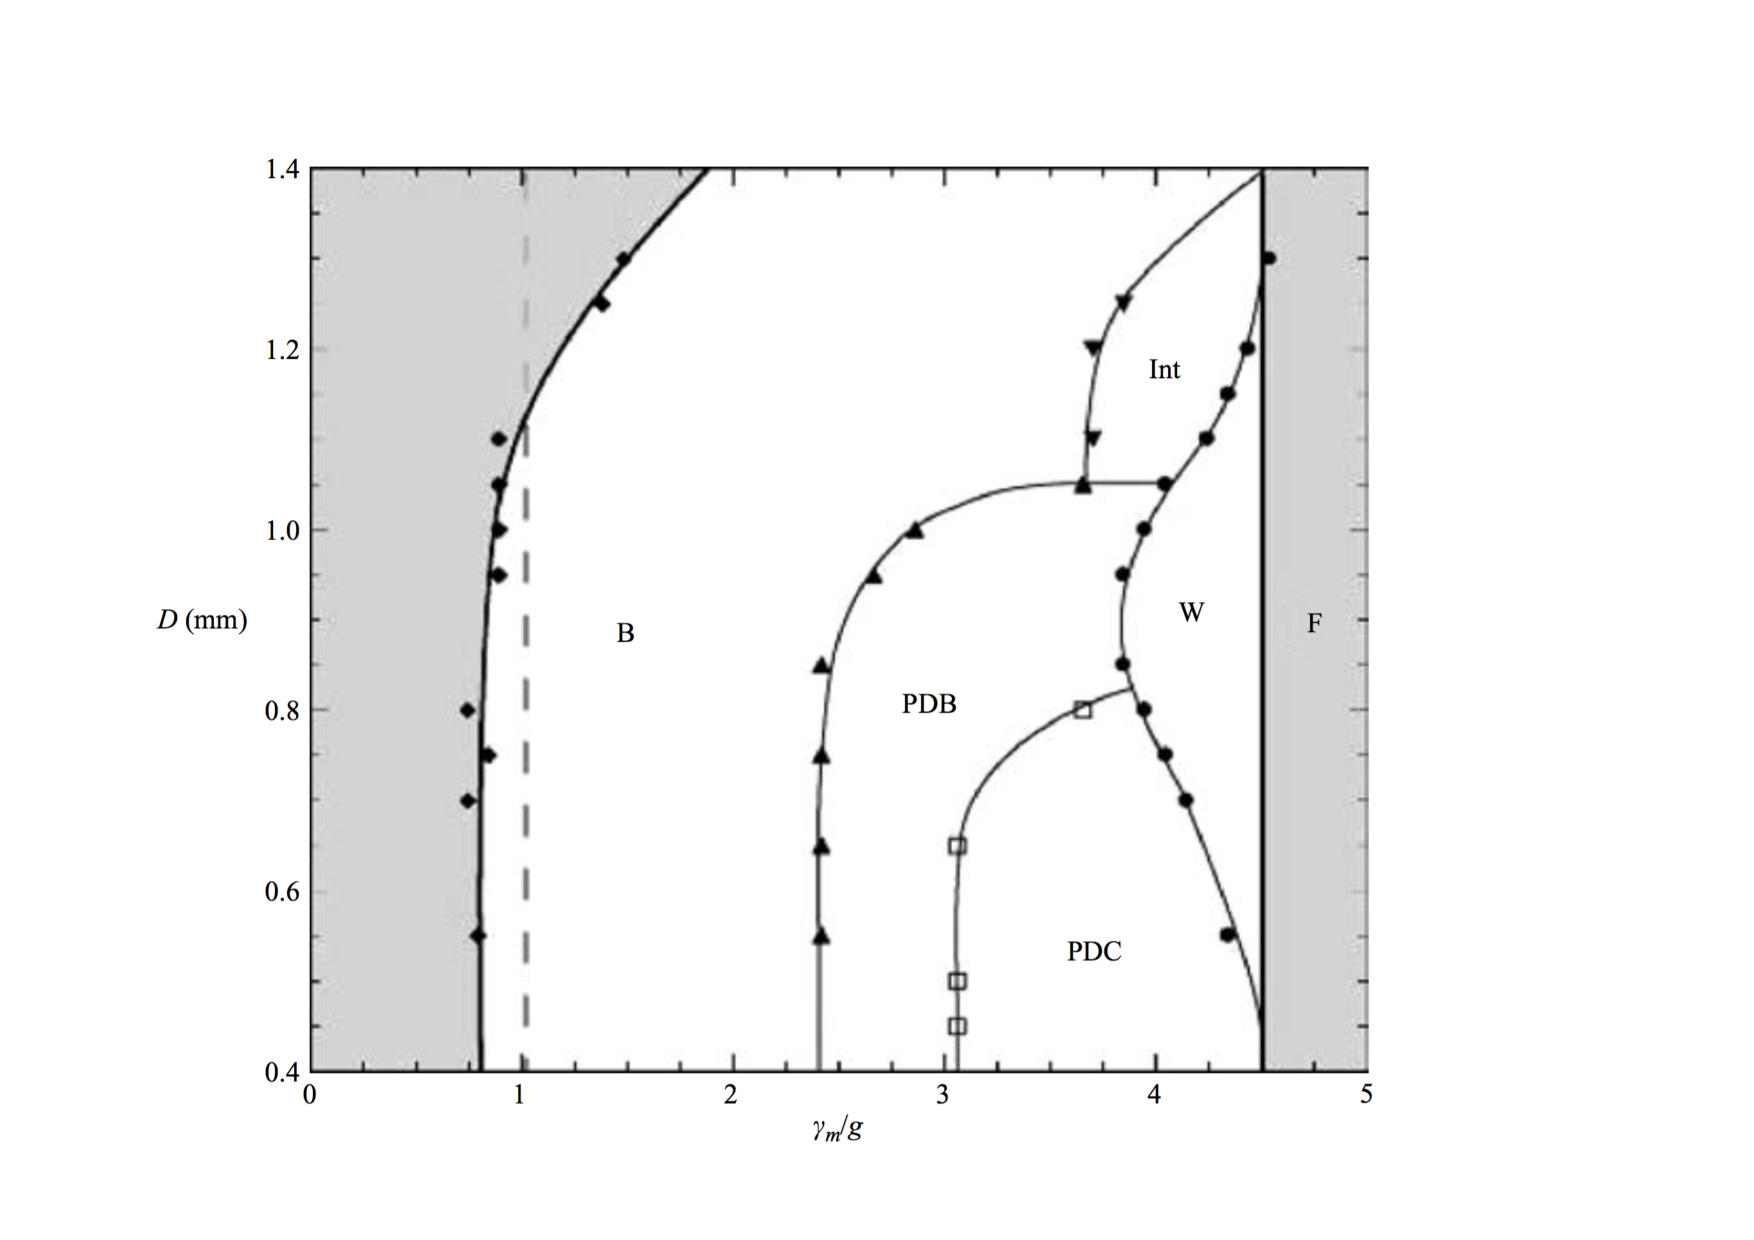
\includegraphics[trim={25mm 15mm 25mm 15mm},clip,width=0.8\textwidth]{PhaseDiagram.pdf}
    \caption{Phase diagram showing the various regimes of a bouncing droplet of silicon oil as a function of the droplet diameter $D$ and $\gamma_m$, with viscocity $\mu_L=\SI{50}{\milli\pascal\second}$ and driving frequency $\SI{50}{\hertz}$.  In B there is simple bouncing, in PDB period-doubling, in PDC transition to temporal chaos by a period-doubling cascade, in Int the drop has an intermittent behaviour, W is the region of walkers and F the Faraday instability domain where Faraday waves are induced on the free surface \cite{9}.}
    \label{figphasediagram}
    \end{figure*}


\subsection{Faraday Waves and Threshold}
\label{secfaradaywavesandthreshold}

% Faraday waves half the driving frequency \cite{15,16}
It is a well known that when subject to an oscillating vertical accelaration the surface of a liquid can become unstable, forming exotic standing waves, known as Faraday waves \cite{20}.  These waves occur with a frequency $f_F$ of half the driving frequency \cite{15}.

% Faraday wavelength from dispersion relation \cite{8,9,15,16}
The wavelength of the Faradays waves $\lambda_F$ can be determined from the dispersion relation of a viscous fluid \cite{8},
\begin{equation}
    \label{disp_rel}
    f_F^2=\left[\frac{g}{2\pi\lambda_F}+\frac{\sigma}{\rho}\left(\frac{2\pi}{\lambda_F^3}\right)\right]\tanh\left(\frac{2\pi h_0}{\lambda_F}\right)
\end{equation}
where $\sigma$ is the surface tension, $\rho$ is the density, $h_0$ is the height of the fluid and $g$ is the acceleration due to gravity.  % \eqref{disp_rel} may be solved for $\lambda_F$ when assumptions about the waves are made.

% Threshold for Faraday waves?

\subsection{Non-coalescent Regimes}
\label{secnoncoalescentregimes}

\subsubsection{Bouncing Droplets}
\label{sec:bouncingregime}

% Brief description of how bouncing occurs (air layer dissapating) \cite{2}
When a droplet of liquid is placed on the surface of the same liquid, coalescence is expected.  There is an instantaneous moment before coalescence where the air layer between the droplet and the fluid interface dissapates \cite{2}.  If the liquid is subject to a vertical oscillation of the form $\gamma(t)=\gamma_m\sin\omega_L t$, where $\gamma_m$ is the maximum acceleration and $\omega_L$ is the angular frequency of oscillation, the droplet lifts off the surface before coalescence, replenishing the air layer.  This periodic dissipating and replenishing of the air layer leads to a stable system of a droplet bouncing on the surface of the liquid.

% Threshold for bouncing \cite{2}

\subsubsection{Walking Regime}
\label{sec:walkingregime}
% Transition to walking (equation of motion) \cite{5,9}
It has been shown that if $\gamma_m$ is increased, various regimes are passed through by the droplet \cite{9}, as shown in \figref{figphasediagram}.  For a certain range of $\gamma_m$, the droplet spontaneously gains a horizontal motion, which may be described by the 1-dimensional equation of motion
\begin{equation}
    \label{eqofmotion}
    m\frac{d^2x}{dt^2}=F^b\sin\left(2\pi\frac{dx/dt}{V_F^\phi}\right)-f^v\frac{dx}{dt}
\end{equation}
where $F^b$ is the force exerted on the drop by the liquid surface, $V_F^\phi$ is the velocity of the Faraday waves and $f^v$ is the effective damping from the dissipation of the air layer.

By seeking steady regimes of the system in the limit of small velocities, it can be shown that the bifurcation threshold $F^b_c$ where the droplet gains horizontal motion is
\begin{equation}
    \label{walkingthreshold}
    F^b_c=f^v\left(\frac{V_F^\phi}{2\pi}\right).
\end{equation}
Above this threshold, the velocity of the walker $V_W$ takes a stable solution of
\begin{equation}
\label{walkervelocity}
V_W=\pm\frac{V_F^\phi\sqrt{6}}{2\pi}\sqrt{\left(F^b-F_c^b\right)/F^b}.
\end{equation}

% PATH MEMORY in background report

\section{Quantum Mechanical Significance}
\label{sec:quantummechanicalsignificance}
It was first noticed by Couder et al.\cite{1} that the system of a walking droplet is reminiscent of one of the early theories of quantum mechanics, the De Broglie-Bohm Theory \cite{17}.  The theory suggests that a particle in a quantum mechanical system is not only acted on by a `classical' potential $V(\bm{r})$, but also by a `quantum-mechanical' potential $U(\bm{r})$ where
\begin{equation}
    \label{qmpotential}
    U(\bm{r})=\frac{-\hbar^2}{2m}\frac{\nabla^2\left|\psi(\bm{r})\right|}{\left|\psi(\bm{r})\right|}
\end{equation}
where $\hbar$ is the reduced Planck's constant, $m$ is the mass of the particle and $\psi(\bm{r})$ is the wave-function of the system.  The evolution of the system can then be described by the equation of motion
\begin{equation}
    \label{qmeqofmotion}
    m\frac{d^2\bm{r}}{dt^2}=-\nabla\left[V(\bm{r})-\frac{\hbar^2}{2m}\frac{\nabla^2\left|\psi(\bm{r})\right|}{\left|\psi(\bm{r})\right|}\right].
\end{equation}

The key concept of the theory is that the evolution of a system is in fact deterministic, with the wave-function `guiding' the particle.  It is here where parallels are draw between this interpretation of quantum mechanics and the system of a walking droplet.  Both systems involve a particle interacting with a wave, a wave that is dependent on the position of the particle.

\section{Macroscopic Quantum Mechanical Observations}
\label{sec:macroscopicquantummechanicalobservations}
As a result of this analogy between a walking droplet and a quantum mechanical particle, experiments have been carried out which subject the walking droplet to macroscopic representations of historically quantum experiments.

\subsection{Single and Double Slits} 
\label{sec:singleandcoubleslits}
It has been shown that when a walker is observed passing through single or double slits, the motion within and after the slit appears to be random \cite{1}.  However, if the statistics of many results are analysed, a familiar distribution for the final trajectory of the walker appears, similar to that of a plane-wave passing through the slit.  The resulting amplitude diffraction pattern for a single slit is
\begin{equation}
    \label{singleslitamplitude}
    f(\alpha)=A\left|\frac{\sin[\pi L\sin(\alpha/\lambda_F)]}{\pi L\sin(\alpha/\lambda_F)}\right|
\end{equation}
where $\alpha$ is the angle subtended by the final trajectory and the path straight through the slit and $L$ is the width of the slit.  For the double slit setup with slit separation $d$, the amplitude diffraction pattern is
\begin{equation}
    \label{doubleslitamplitude}
    f(\alpha)=A\left|\frac{\sin\left[\pi L\sin(\alpha/\lambda_F)\right]}{\pi L\sin(\alpha/\lambda_F)}\cos\left[\pi d\sin(\alpha/\lambda_F)\right]\right|.
\end{equation}
These distributions are similar to a quantum-mechanical particle passing through single or double slits ($\lambda_F$ is replaced by the De Broglie wavelength), demonstrating the similarities between a walker being guided by its Faraday wave and a quantum particle being guided by its wave-function.

\subsection{Orbital Quantisation and Splitting}
\label{sec:orbitalquantisationandsplitting}
Following this quantum-like behaviour of walkers in single and double slit experiments, it was also shown that two walkers can enter into stable orbits, with discrete orbital diameters $d_n$ given by
\begin{equation}
    \label{orbit}
    d_n=(n-\epsilon_0)\lambda_F
\end{equation}
where $\epsilon_0$ is a constant and $n=1,2,3,\ldots$ for in-phase bouncing of the droplets and $n=1/2,3/2,5/2,\ldots$ for anti-phase bouncing \cite{5,9,6}.

\begin{figure}[h]
    \centering
    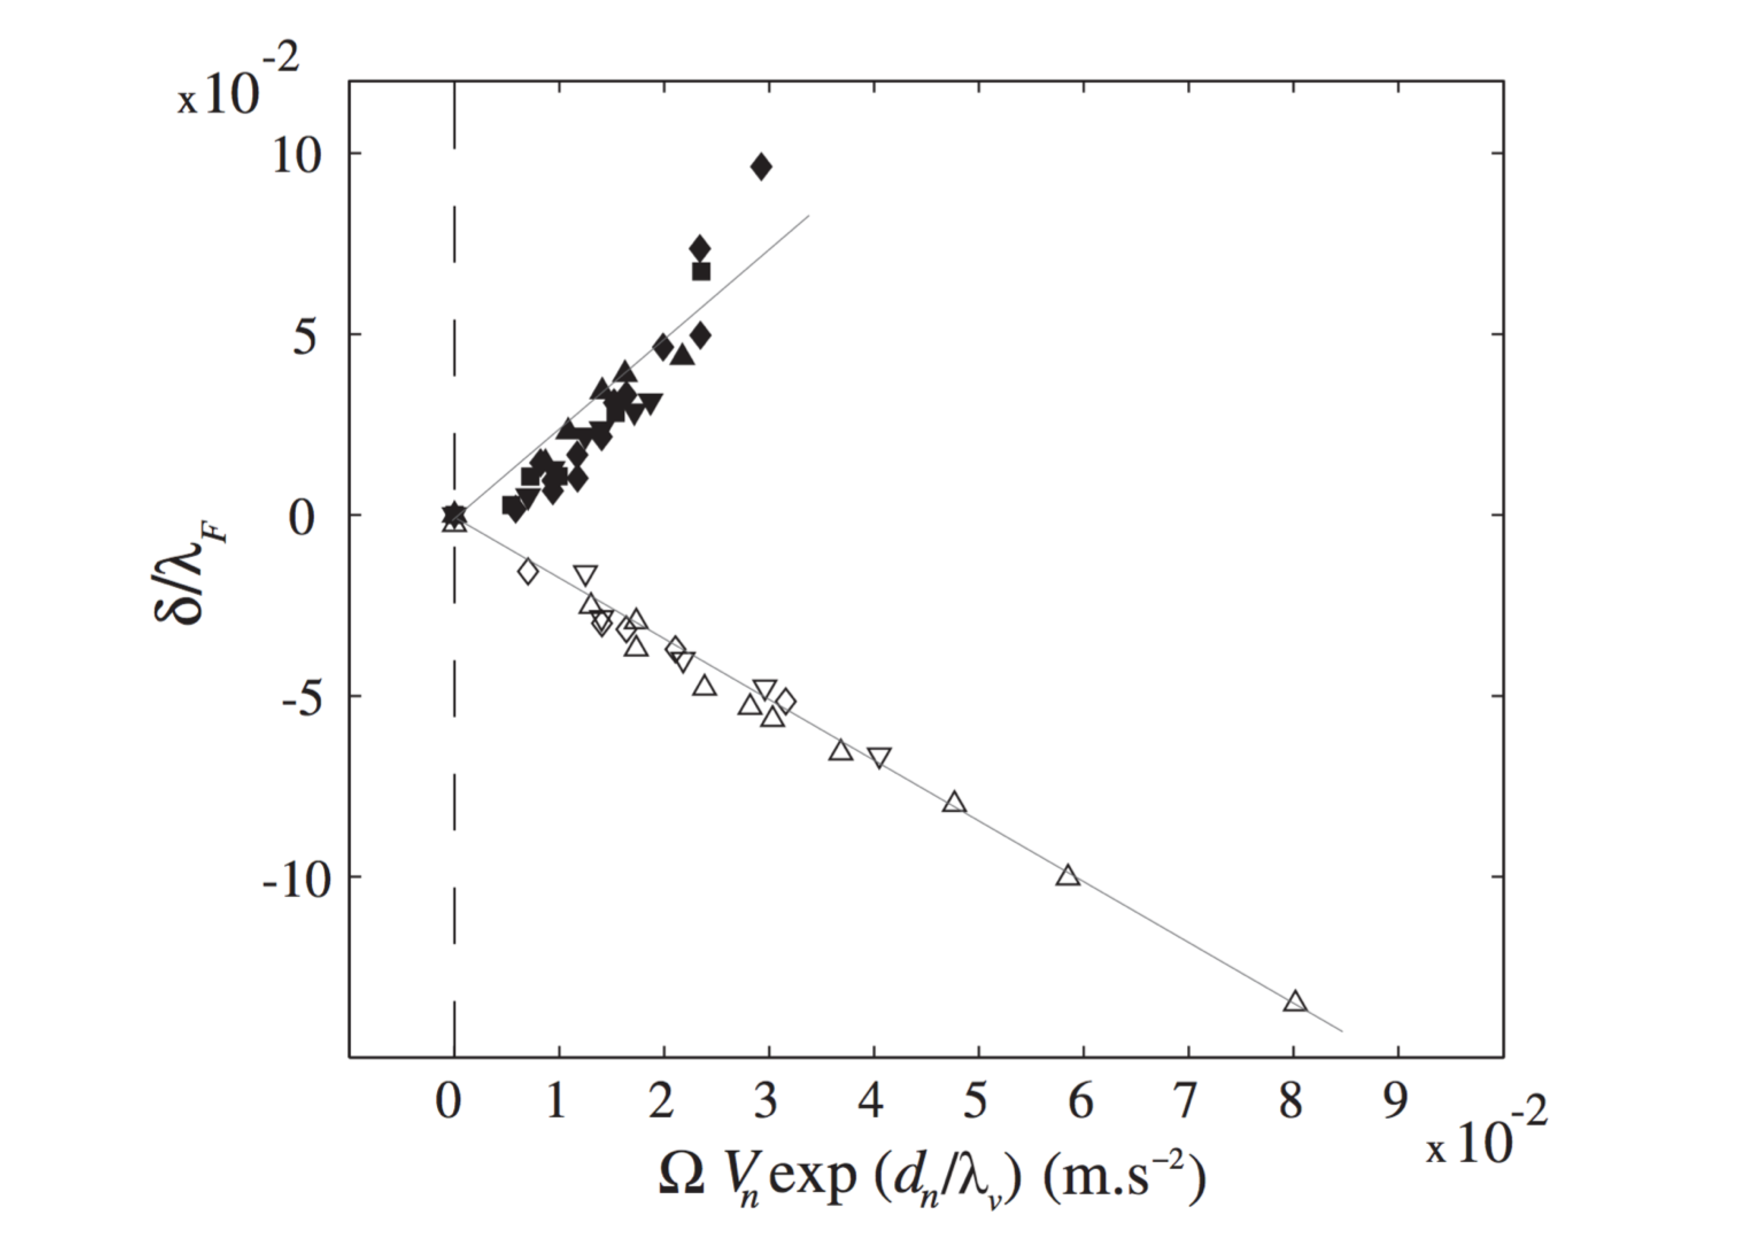
\includegraphics[width=\columnwidth]{LevelSplitting.pdf}
    \caption{The splitting $\delta$ of the orbitals as a function of the angular velocity $\Omega$.  Here, $V_n$ is the velocity of the walker in the $n^{th}$ orbit and $\lambda_v=\lambda_F$.  The solid data points are corotating walkers and the hollow points counterrotating walkers.}
    \label{fig:levelsplitting}
\end{figure}

This quantum-like orbital quantisation led to the further investigation of this system when a force is applied; in this case the Coriolis force due to rotating the bath \cite{6}.  As the rotation of the bath is increased, a linear splitting of the orbitals is seen, with corotating\footnote{walkers orbiting the same direction to the rotation of the bath.} walkers increasing their orbital diameter and counterrotating\footnote{walkers orbiting in the opposite direction to the rotation of the bath.} walkers decreasing their diameter, as shown in \figref{fig:levelsplitting}.  It is shown that there is a relationship between the vorticity $\bm{\Omega}$ and the fluid velocity $\bm{U}$,
\begin{equation}
    \label{vorticity}
    2\bm{\Omega}=\bm{\nabla}\times\bm{U},
\end{equation}
which corresponds to $\bm{B}=\bm{\nabla}\times\bm{A}$ from electromagnetism, where $\bm{B}$ is the magnetic field and $\bm{A}$ is the magnetic vector potential.  Hence, this system is demonstrated to be a macroscopic analogy of Zeeman splitting of atomic levels when subject to an external magnetic field.

% \subsection{Barrier Tunnelling}
% \label{sec:barriertunnelling}
% \cite{7}
% Walkers have also been shown to escape confinement and pass through barriers in a quantum-like, probabilistic manner \cite{7}.  The barriers were created by altering the depth of the silicon oil bath which, as shown by \eqref{walkervelocity}, directly effects $V_W$, as $V_W=V_W(h)$.  It is seen that the probability of escape of a walker depends on $V_W$ and the barrier thickness, creating a system analogous to an alpha particle exhibiting quantum tunnelling to escape from a nucleus.
% key results, dependence of probability on V and barrier height
% no equations needed

\subsection{Particle statistics in a Corral}
\label{sec:particlestatisticsinacorral}
\begin{figure}[h]
	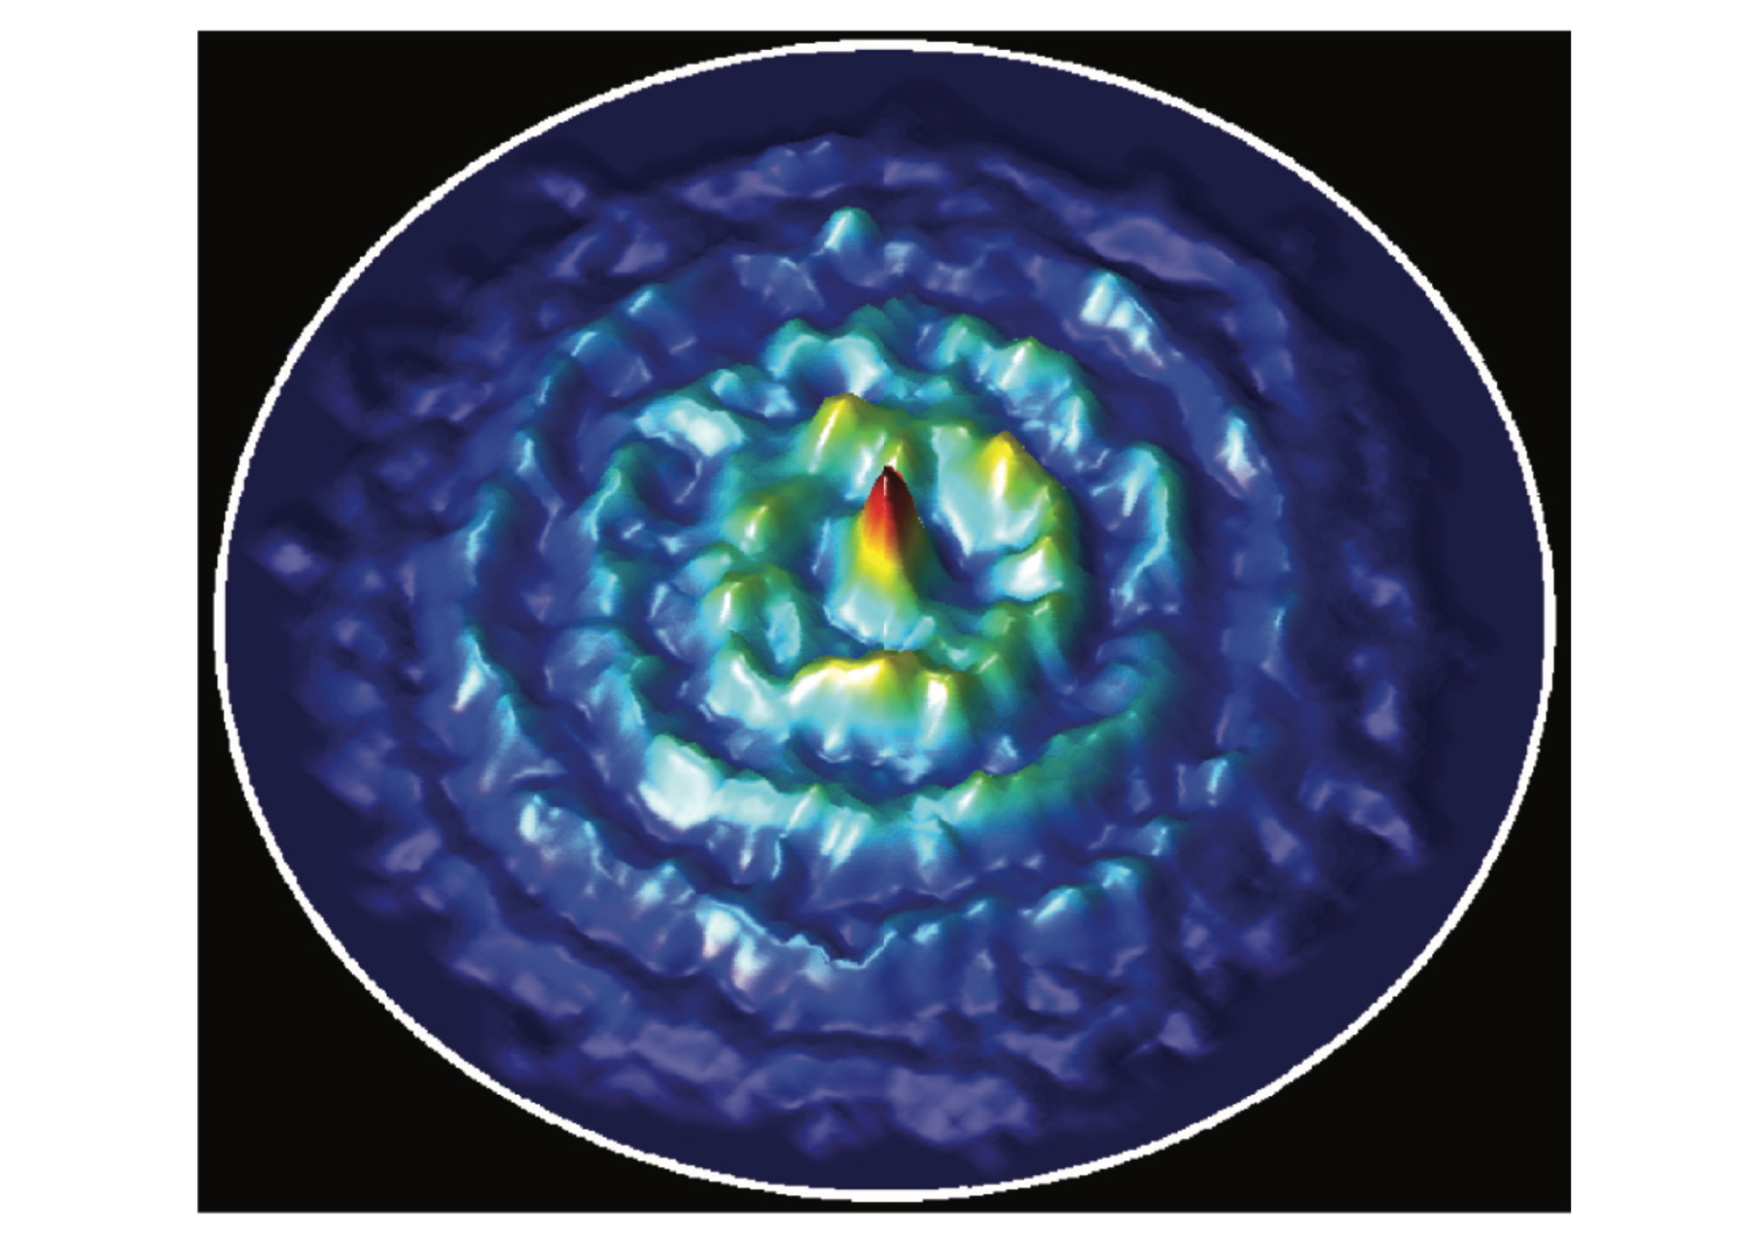
\includegraphics[width=\columnwidth]{WalkerCorral.pdf}
	\caption{Probability distribution of a walking droplets position when confined to a circular corral \cite{12}.}
	\label{fig:walkercorral}
\end{figure}

\begin{figure}[h]
	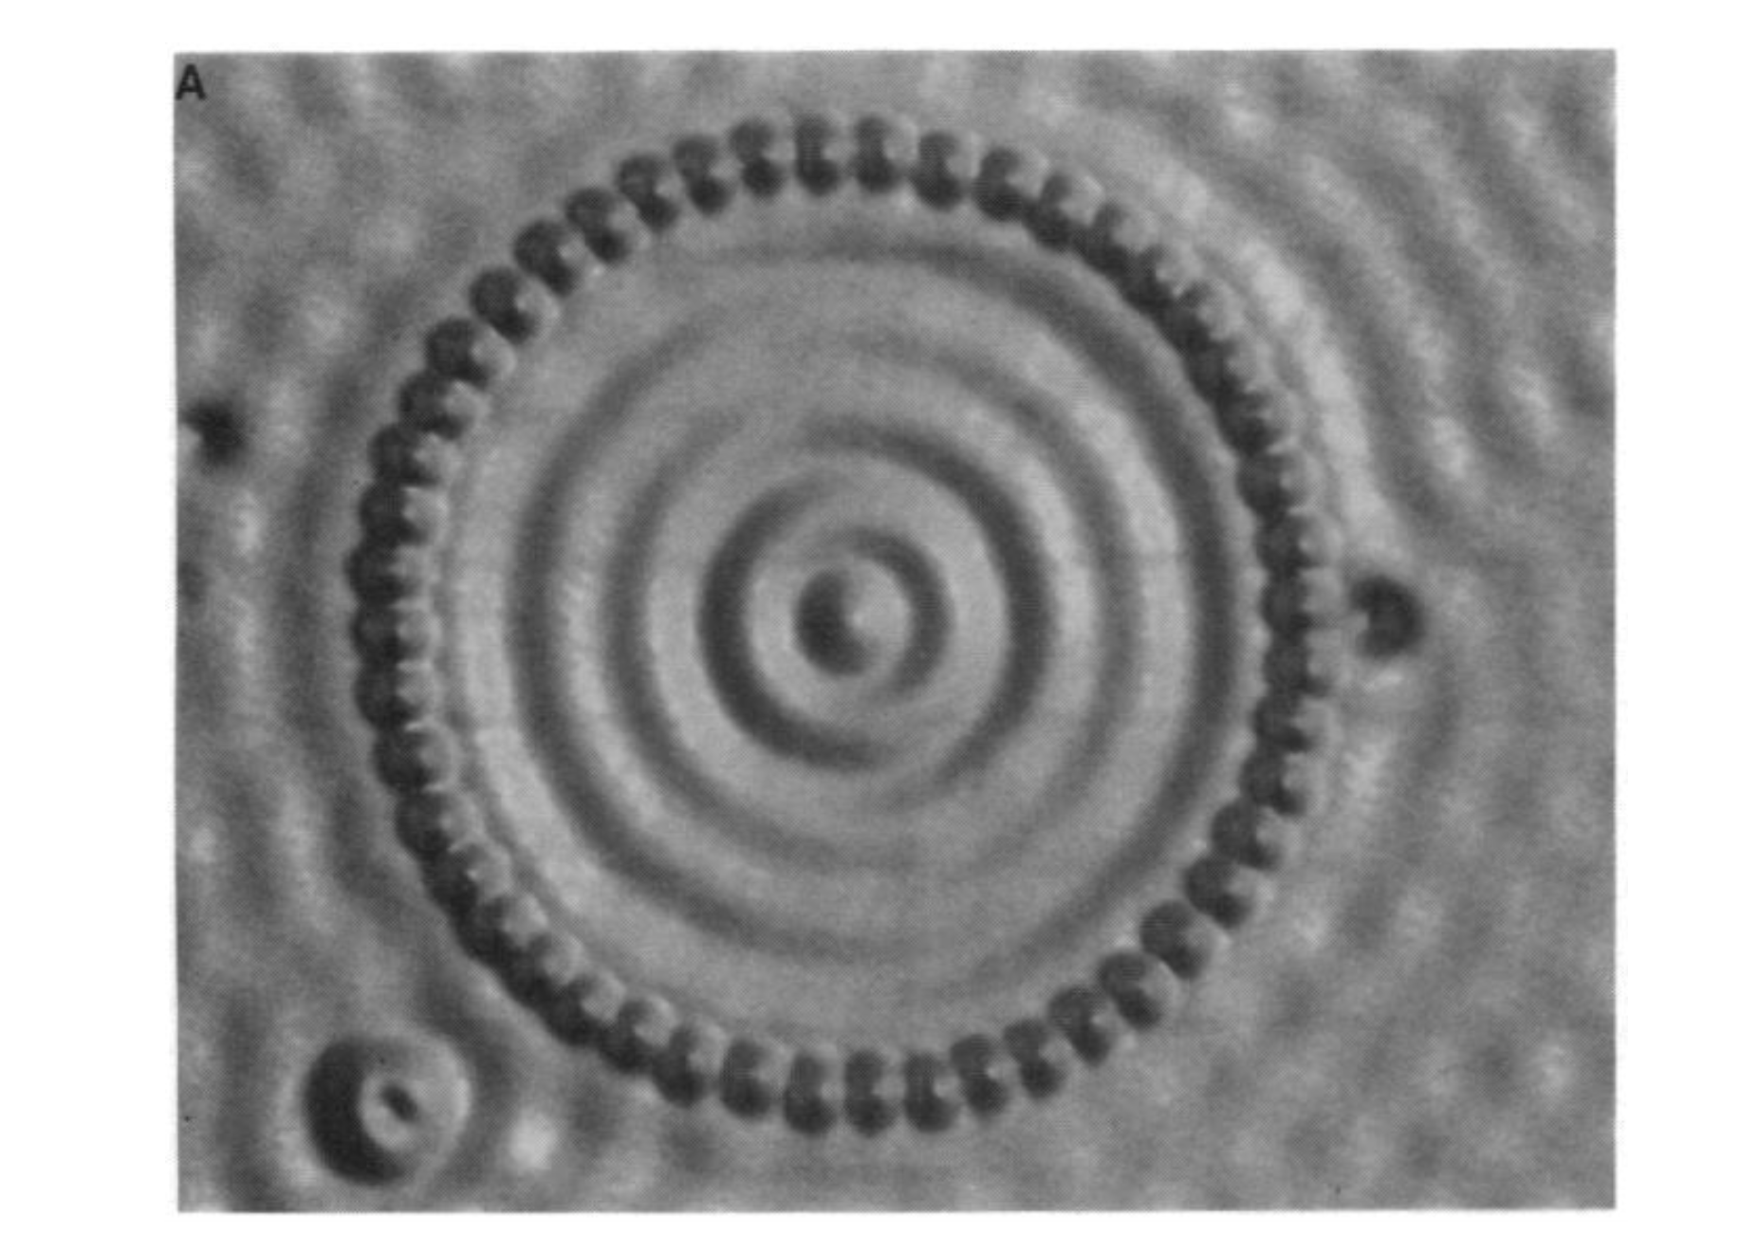
\includegraphics[width=\columnwidth]{ElectronCorral.pdf}
	\caption{Spatial image of the eigenstates of a quantum corral \cite{21}.}
	\label{fig:electroncorral}
\end{figure}

An experiment carried out by J. Bush et al. \cite{12} has shown that in the long path memory limit, a walkers motion when confined by a corral becomes complex and seemingly random.  A build-up of the walkers position with time however shows that it may depend on the Faraday mode of the corral; the solution to the wave equation with the correct boundary conditions (\figref{fig:walkercorral}).  This statistical dependence of the walker can be compared to the density of states of a two-dimensional electron gas confined to a quantum corral \cite{21}, where measured eigenstates of the corral agree well with those predicted by solving the Schr{\"o}dinger equation for such a corral, as seen in \figref{fig:electroncorral}.

\section{Proposed Experimental}
\label{sec:proposedexperiment}
The proposed experiment is to further the work of J. Bush et al. in investigating the statistics of walkers confined to corrals with dimensions comparable to $\lambda_F$.  This will be done by inducing walkers in corrals filled with silicon oil, as used in previous experiments, which are subject to a vertical oscillation.  A variety of corral geometries will be investigated, including the original circular corral, ensuring that previous results can be realised \cite{12}.

The predicted outcome is that the statistics of walkers within simple corrals will remain related to the Faraday modes of the corrals.  It is expected that this relationship will also depend heavily on the exact shape of the corrals.

A numerical model of the walker-corral system will also be created, allowing the testing of small variations in the corral geometries.

A comparison of this experimental and simulated data with known quantum systems will provide further testing of the analogy between a walker and a quantum-mechanical particle.

\bibliographystyle{ieeetr}
\bibliography{references} 

\end{document} 
